\documentclass{article}

% Section has a dot
\usepackage{titlesec}
  \titlelabel{\thetitle.\quad}

% Add image
\usepackage{graphicx}

% Dot-filling for ToC's Sections
\usepackage{tocloft}
\renewcommand\cftsecleader{\cftdotfill{\cftdotsep}}

% For pseudocode
\usepackage[linesnumbered,ruled]{algorithm2e}

\title{Chapter 4 Exercises}
\date{2019-08-06}
\author{Termanteus}

\begin{document}

\maketitle
\pagenumbering{gobble}
\newpage
\pagenumbering{arabic}
\tableofcontents
% --------------------- LAYOUT ---------------------
\newpage \section{R-4.1}
\paragraph{Statement}
Describe a recursive algorithm for finding the maximum element in a sequence, S, of n elements. What is your running time and space usage?
\paragraph{Solution}
  Both running time and space usage are O(n)
  \begin{algorithm}[h!]
    \SetKwInOut{Input}{Input}
    \SetKwInOut{Output}{Output}
    
    \underline{function findMax} $(S,n)$\;
    \Input{Array of numbers, n}
    \Output{Maximum value from 0 to n in the array S}
    \If{$n == 1$}{
      \KwRet{$S[n-1]$}\;    
      }
      $currentMax \longleftarrow findMax(S,n-1)$\;
    \eIf{$currentMax > S[n-1]$}{
      \KwRet{$currentMax$}\;
      }{
      \KwRet{$S[n-1]$}\;
      }
    \caption{Recursive algorithm for finding maximum}
  \end{algorithm}
\newpage \section{R-4.2}
\paragraph{Statement}
Describe a recursive algorithm for finding the maximum element in a sequence, S, of n elements. What is your running time and space usage?
\paragraph{Solution} Picture
\begin{figure}[h!]
  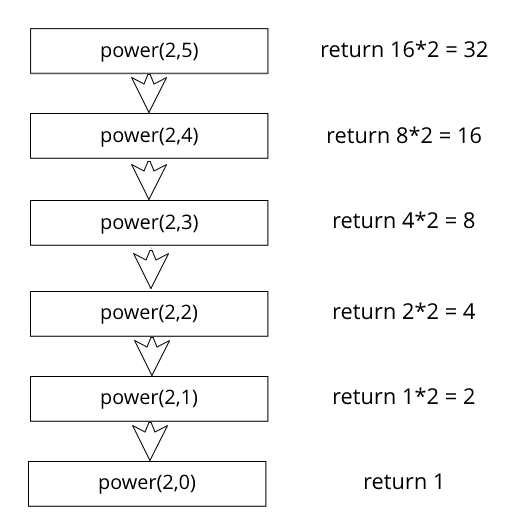
\includegraphics[width=\linewidth]{Drawing.png}
  \caption{Power(2,5) of Code Fragment 4.11}
  \label{fig:Power(2,5)}
\end{figure}


\section{R-4.3}
  Skip because of the drawing...
\section{R-4.4}
  Skip because of the drawing...
\section{R-4.5}
  Skip because of the drawing...
\section{R-4.6}
  \paragraph{Statement}
  Describe a recursive function for computing the $n^{th}$ Harmonic number $H_{n}=\sum_{i=1}^{n}{\frac{1}{n}}$.
  \paragraph{Solution}
    Pseudocode
    \begin{algorithm}[h!]
      \SetKwInOut{Input}{Input}
      \SetKwInOut{Output}{Output}
      
      \underline{function harmonicNumber} $(n)$\;
      \Input{Index n}
      \Output{The n-th value in Harmonic Number}
      \If{$n == 1$}{
        \KwRet{$1$}\;    
        }
      \KwRet{$ \frac{1}{n} + harmonicNumber(n-1)$}\;
      \caption{Compute the n-th \textbf{Harmonic number}}
    \end{algorithm}
\section{R-4.7}
  \paragraph{Statement}
  Describe a recursive function for converting a string of digits into the integer it represents. For example, 13531 represents the integer 13,531.
  \paragraph{Solution}
    Pseudocode
    \begin{algorithm}[h!]
      \SetKwInOut{Input}{Input}
      \SetKwInOut{Output}{Output}
      
      \underline{function toInt} $(string,i)$\;
      \Input{String of digits, current index}
      \Output{Number of the string represents until character i }
      \lIf{$i == 1$}{
        \KwRet{int(string[i])}
      }
      \lIf{$i == 0$}{
        \KwRet
      }
      \KwRet{$ toInt(string, i - 1) * 10 + int(string[i])$}\;
      \caption{Convert a string of digits into the integer it represents}
    \end{algorithm}
\section{R-4.8}
  \paragraph{Statement}
  Isabel has an interesting way of summing up the values in a sequence A of n integers, where n is a power of two. She creates a new sequence B of half the size of A and sets $B[i] = A[2i]+A[2i+1]$, for $i = 0,1,...,(n/2)-1$. If B has size 1, then she outputs $B[0]$. Otherwise, she replaces A with B, and repeats the process. What is the running time of her algorithm?
  \paragraph{Solution}
    \textbf{Total Running time:} O(n)\par
    There're total of $log_{2}n$ recursive calls. But in the first run, this algorithm has already had to make n/2 = O(n) sums, that also the cost for creating sequence B or re-set A = B.
\section{C-4.13}
  \paragraph{Statement}
  In Section 4.2 we prove by induction that the number of lines printed by a call to draw\_interval(c) is $2^c -1$. Another interesting question is how many dashes are printed during that process. Prove by induction that the number of dashes printed by draw\_interval(c) is $2^{c+1}-c-2$. 
  \paragraph{Solution}
  P(c): The number of dashes printed by draw\_interval(c) is $2^{c+1}-c-2$.\par
  \textbf{Base case}: P(1): 1 dash is drawn. Correct.\par
  \textbf{Inductive step}: Assume P(n) is True. Prove P(n+1) true.\par
  draw\_interval(n+1) will call draw\_interval 2 times and draw\_line(n+1) 1 time.\par
  For each draw\_interval(n): $2^{n+1}-n-2$ dashes is drawn.\par
  For draw\_line(n+1): $n+1$ dashes is drawn.\par
  Total: $2^{n+1}-n-2 + 2^{n+1}-n-2 + n +1 = 2^{c+2} - c - 3$. P(n+1) holds.\par
  \textbf{Proved.}
  \end{document}